\def\thesection {\arabic{section}}
\introduction*{Note Introduttive}
\addcontentsline{toc}{chapter}{\protect\numberline{}{Note Introduttive}}
\markboth{Note Introduttive}{pagenumber}
%\endinput

\noindent Al termine {\em Meccanica} non corrisponde una sola disciplina. Il dominio
abbracciato da questa materia \`e assai vasto e una classificazione, forse leggermente
arbitraria e imprecisa, sicuramente incompleta,
dispone questa parte della {\em Fisica} in quattro branche, a loro volta molto estese:
la {\em Meccanica Classica}, la {\em Meccanica Statistica},
la {\em Meccanica Relativistica} e la {\em Meccanica Quantistica}. Questi quattro rami,
i nomi dei quali si apprendono, unitamente ai loro principali risultati,
nel corso della formazione
secondaria, sono tra loro intrecciati: \`e comune trovare, nelle librerie
scientifiche, trattati di {\em Meccanica Quantistica Relativistica}
oppure di {\em Meccanica Statistica  Relativistica}.

\noindent Prendendo le mosse da \cite{finzi},
se si volesse rispondere alla domanda ``che cos'\`e la {\em Meccanica}?''
 si potrebbe dire:
essa si propone lo scopo di descrivere i movimenti che avvengono nello spazio e nel
tempo in relazione alle cause che provocano tali moti; 
definizione che ognuno vede quanto sia ampia. Infatti, tutte
le interazioni fisiche, avendo luogo
nello spazio e nel tempo, implicano {\em movimento}. Prendendo quindi tale definizione
per  buona, la {\em Meccanica} dilagherebbe in quasi tutti i campi della {\em Fisica}. 
D'altra parte, i fenomeni naturali appartengono a tutte le branche della {\em Fisica} e,
a rigore, sta a chi si occupa di tali problemi decidere di trascurare
certuni o cert'altri aspetti. 
Quando, nello studio del movimento, sono trascurabili o vengono trascurati
gli scambi e le variazioni termiche, le relazioni elettromagnetiche,
chimiche, nucleari e non si palesano velocit\`a prossime a quelle della luce
ricadiamo, in generale, 
nell'ambito della Meccanica Classica\index{meccanica classica}.

\noindent Limitandoci quindi alla branca della Meccanica Classica avremo una copiosissima
biblioteca di opere importanti e ispiratrici, se non altro come fonti del
modello espositivo {\em standard} dell'introduzione alla {\em Cinematica},
modello che, per ragioni che cercher\`o di esporre
pi\`u avanti, non seguiremo.
\noindent Riporto soltanto due trattati di Meccanica Classica, 
ben conscio per\`o di proporre
una  porzione minuscola della letteratura effettivamente disponibile in questo campo. 
Sia \cite{goldstein} sia \cite{levicivita} entrano in argomento definendo e descrivendo il
moto di un punto. Come anticipato, non sar\`a per\`o questo il nostro {\em incipit}. Uno 
dei motivi che mi hanno persuaso a non cominciare lo studio della Meccanica
dalla cinematica del punto riguarda il fatto
che il concetto di velocit\`a angolare compare in questo studio in
modo forzato, tramite
altri oggetti, in quanto sui punti non si possono misurare angoli. Ma il motivo 
principale, che da solo potrebbe bastare a farci prendere un'altra strada, \`e che,
pur riconoscendo allo studio della cinematica del punto un notevole valore
formativo, tale studio ci sembra fuorviante dal solco maggiormente
 aderente alle applicazioni
tecniche della Meccanica, che \`e la traccia che invece
vorremmo seguire in questo spazioso campo.

\noindent Il nostro percorso, infatti, si snoder\`a tra le {\em macchine} e i loro componenti: esse saranno studiate
utilizzando i metodi di indagine, i risultati, e quanto possibile dell'impianto
concettuale e del complesso di idee che formano la Meccanica Classica,
scienza con vocazione prevalentemente matematica. Evitando
di entrare in un secondo girone di definizioni che rispondono a ``cosa sono le macchine?'',
desiderosi anzi di toglierci quanto prima da tali gineprai,
baster\`a qui dire che non esistono macchine o parti di esse che siano punti isolati.
Sicuramente la nozione di {\em punto} \`e fondamentale, intuitiva e presa volentieri
in prestito, ringraziando, dalla geometria. Ma il punto, nella nostra trattazione,
apparterr\`a sempre a un corpo o, pi\`u precisamente, a una entit\`a
che definiremo come {\em corpo rigido}
\index{corpo rigido} e che sar\`a il protagonista dei nostri moti. Partiremo quindi
dallo spostamento dei corpi, come in \cite{whittaker}. I risultati e le conclusioni
ai quali giungeremo saranno comunque in sintonia
con tutte le altre trattazioni della Meccanica.

\section{Cenni Storici}
Riprendiamo nel presente paragrafo quanto riporta \cite{finzi} nella sua introduzione, opera
insigne, questa, che l'autore ha avuto la fortuna di dover studiare per
preparare l'esame di {\em Meccanica Razionale}.
Pare che, prima dell'intervento leonardesco, pochi autori si fossero espressi,
e soltanto in considerazioni filosofiche, sulle cause del moto e sulle condizioni di
equilibrio, seguendo i resti della Filosofia Greca conservata e giunta in Europa
con l'eredit\`a della ``Scuola Alessandrina''. Tra i diversi
frammenti, a noi pervenuti da tale ``patrimonio'', segnaliamo
un'opera preziosa per chi volesse esplorare le sorgenti del
pensiero scientifico: \cite{aristotele}.
{\em Leonardo da Vinci} apr\`i il primo sentiero, per lo studio della Meccanica,
pressoch\'e scevro 
dai pregiudizi della Filosofia Antica e dalle opinioni teologiche, tanto autorevoli
e tanto in voga durante i secoli precedenti.
Il periodo moderno della Meccanica ha per\`o inizio con le nuove concezioni 
circa il moto dei pianeti elaborate da {\em Copernico} e {\em Keplero}; 
e tali idee
portarono un radicale sconvolgimento nel campo dell'astronomia.
\`E appena posteriore a questa notevolissima ``riforma astronomica'' la fondazione,
da parte di {\em Galileo}, 
del cosiddetto {\em metodo di indagine sperimentale}, che
negli ultimi tre secoli \`e stato spesso indicato come l'unica strada
sicura per il progresso della Scienza.
{\em Galileo} formula per primo la nozione precisa di
accelerazione e intuisce che questa grandezza dovr\`a comparire tra i protagonisti sul
palcoscenico della Meccanica. Nel frattempo {\em Cartesio} pone le basi
esatte per lo studio quantitativo della geometria e, siccome il
movimento dei corpi ha luogo
nelle dimensioni dello spazio, forgia alcuni strumenti
che renderanno il cammino della Meccanica pi\`u rapido,
 {\em in primis} la
{\em Geometria Analitica}.
Su queste solide fondamenta si sviluppano alcuni rami della {\em Statica},  
per opera di {\em Varignon} e {\em Stevin},
e tali studi -- senza dimenticare quelli pionieristici e ancora fondamentali
di {\em Archimede} -- costituiscono ancora oggi un notevole bagaglio di sapere tecnico.
\begin{wrapfigure}{r}{0.5\textwidth}
	  \begin{center}
	  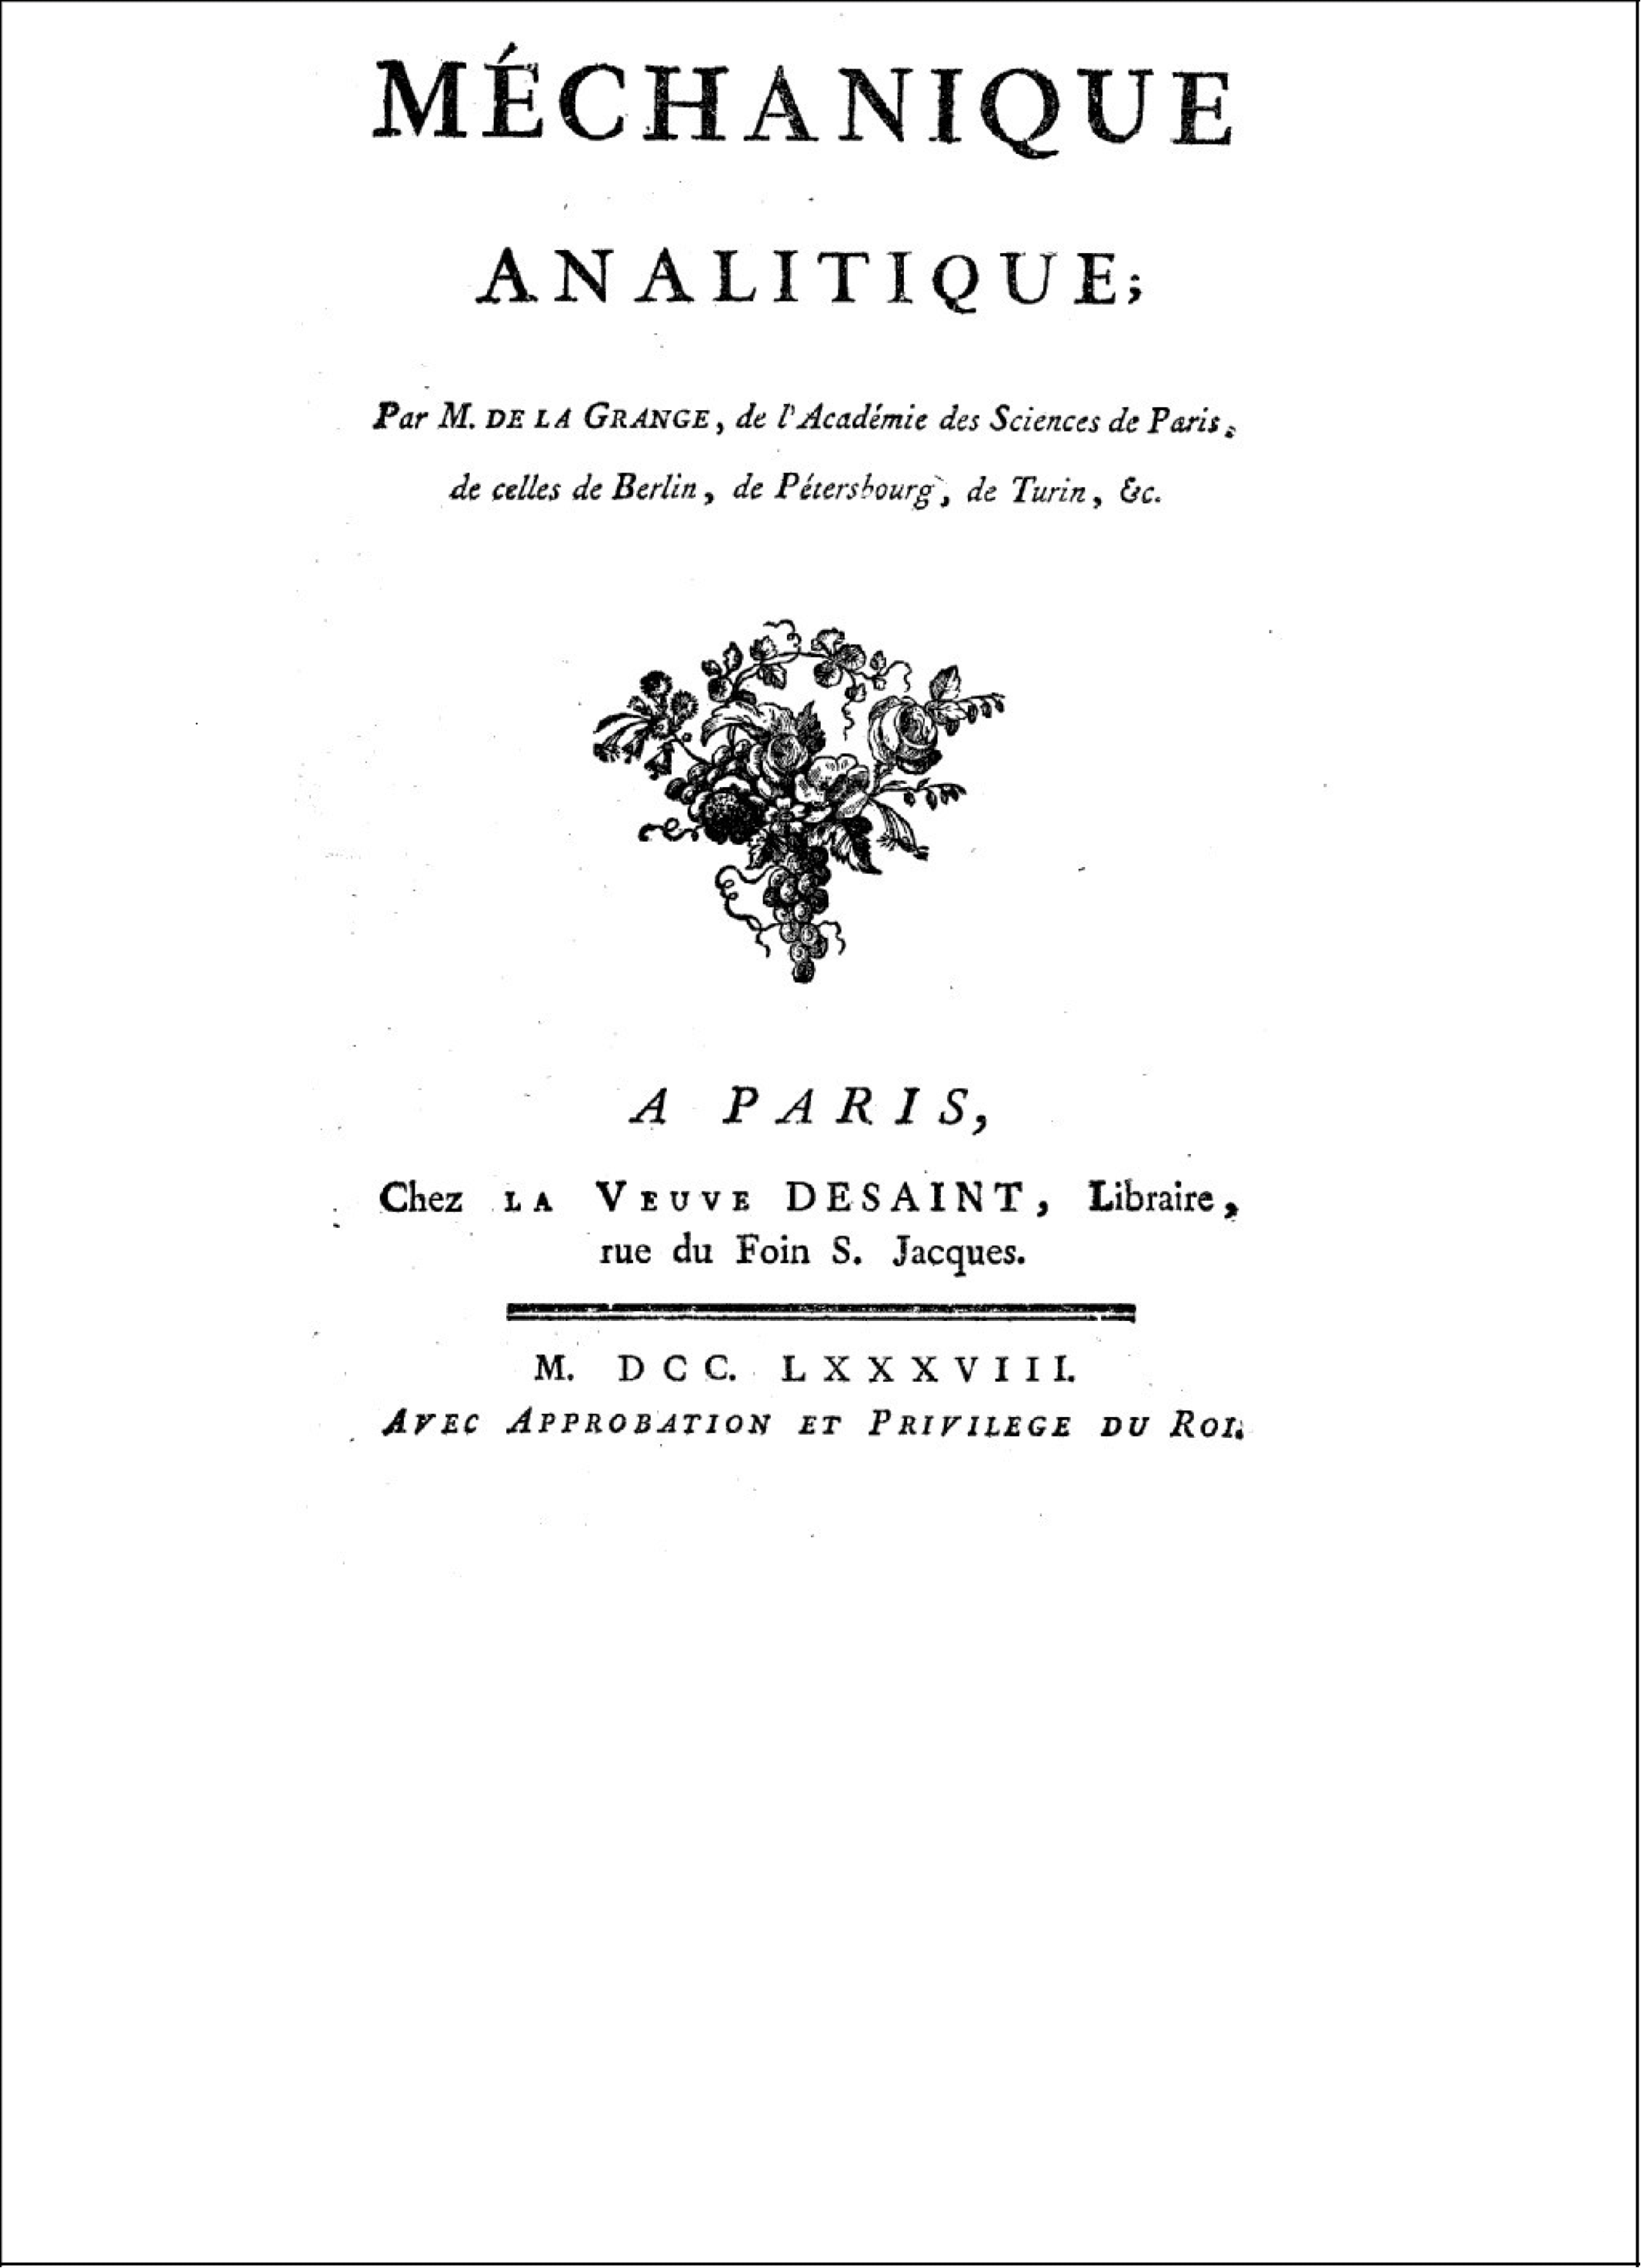
\includegraphics[width=0.42\textwidth]{part0/FIG/mechanique.pdf}
	  \end{center}

	  {\em Il frontespizio del libro di Lagrange.}
\end{wrapfigure}
\noindent La definitiva sistemazione della legge d'inerzia (gi\`a intravista da
{\em Galileo}) da parte di {\em Newton} e il ``suo''
{\em Calcolo Infinitesimale}\footnote{
{\em Philosophi\ae Naturalis Principia Mathematica}, 1687, opera non visionata dall'autore.
}
dotano il secolo XVIII di strumenti per affrontare un ventaglio amplissimo
di problemi di meccanica. Nel corso di quel secolo, i
{\em Bernoulli} ({\em Giacomo}, {\em Giovanni} e {\em Daniele})
prima, {\em Eulero}  poco dopo, raffinando ulteriormente 
i concetti dell'Analisi Matematica,
posero le basi per quello che oggi si chiama
{\em Calcolo delle Variazioni}. Essi impostarono 
correttamente e risolsero svariati
problemi paradigmatici di statica e di dinamica. Ormai il {\em Principio dei Lavori
Virtuali} aveva ottenuto una formulazione precisa e {\em Monsieur de la Grange}, noto
poi come {\em Lagrange}, scriveva il suo bel trattato {\em M\'echanique Analitique}
(il cui frontespizio appare qui a lato) nel
quale, facendosene un curioso vanto, non inser\`i alcuna figura.
{\em Lagrange} portava cos\`i a compimento e sintetizzava  quel dovizioso
novero di metodi matematici disponibili  
alla fine del secolo XVIII.
Al termine di tale secolo, la Meccanica si trova ormai ripartita
in diversi rami dovendo fornire risposte a specifiche
necessit\`a dei vari ambiti applicativi, vertiginosamente
crescenti con l'avvento della Rivoluzione Industriale:
problemi di
{\em elasticit\`a}, di {\em idrodinamica}, di {\em suono} e {\em vibrazioni}, di
{\em meccanica delle macchine}. 

\noindent \`E proprio durante il secolo XIX che la Meccanica subisce, a livello teorico, ulteriori
e ``definitive'' sistematizzazioni dovute a {\em Laplace}, {\em Gauss}, {\em Cauchy}
e {\em Hamilton}, nonch\'e alcune importanti rivisitazioni critiche per opera di {\em 
Poincar\'e}, {\em Hertz} e soprattutto {\em Mach}. A stimolare la revisione dei
fondamenti
di questa scienza sono prevalentemente il concetto di {\em forza} e di
{\em spazio} e
{\em tempo assoluti}. {\em Mach}, nel suo prezioso libro \cite{mach}, 
prepara il terreno per la Meccanica Relativistica di {\em Einstein}, che dovr\`a 
entrare poi in quasi tutte le branche della Fisica. Consiglio agli
appassionati di meccanica, di scienza e di tecnica una lettura di \cite{mach}, se
non altro
per rendersi conto di quanto un pensiero, molto indipendente e rigoroso, possa mettere
in discussione qualsiasi teoria che, per et\`a, per diffusione, per abbondanza di
risultati, tenda al dogmatismo.

\noindent Oltre a questo, come si \`e gi\`a accennato, il secolo XIX porta alla
ribalta le esigenze della nascente Rivoluzione Industriale. La Meccanica scopre
allora la propria vocazione {\em applicativa}. Alcuni dei frutti delle ricerche svolte da
{\em Poisson}, {\em Cauchy}, {\em Carnot}, {\em Coriolis} sono squisitamente
applicativi e appartengono alla {\em Meccanica Applicata}. 
Questa, a sua volta, si \`e occupata e si occupa di un 
campo molto esteso di problematiche. Si va dalla {\em Statica} dei corpi all'{\em
Elasticit\`a}, studi che ormai spettano alla {\em Scienza delle Costruzioni},
si procede con la {\em Meccanica dei Fluidi}, di estremo interesse
per gli ingegneri civili quando il fluido \`e l'acqua e per gli ingegneri aeronautici quando
il fluido \`e l'aria. Si spazia poi dall'{\em Acustica} alle {\em Vibrazioni}, dalla
{\em Biomeccanica} alla moderna {\em Balistica}.

\noindent Giungiamo  quindi alle {\em Macchine}, con i loro organi e i loro azionamenti, 
i loro movimenti speciali, le loro 
criticit\`a e la loro straordinaria rilevanza economica.
Eccoci all'imbocco di una nuova restrizione del campo di questa
scienza; \`e l'unico strato che riguarder\`a da vicino la materia del
nostro corso. 
Anzi, nel dominio stesso della meccanica delle macchine, saremo portati o costretti
a fare delle scelte che, per forza di cose, limiteranno ulteriormente 
lo scopo di queste note.

\section{Il Nostro Approccio alla Meccanica delle  Macchine}
Questo lavoro si rivolge, in particolare, agli studenti dei corsi di
Ingegneria che prevedono l'insegnamento della Meccanica Applicata alle Macchine.
Alcuni di tali corsi non sono preceduti
da insegnamenti che abbraccino argomenti di meccanica,
fatta eccezione per l'insegnamento
della fisica del primo anno. Si rende cos\`i necessario anteporre alle
nozioni di {\em Cinematica Applicata}, contenute nella {\em Seconda Parte} e
approfondite nella {\em Terza Parte}
di questo volume, un'introduzione alla {\em Cinematica Teorica}.
La {\em Prima Parte}, infatti, richiama
i concetti di {\em corpo rigido} e di {\em moto relativo},
proponendo anche alcune nozioni circa la composizione
dei movimenti. Come gi\`a accennato, partiremo dal concetto di 
{\em velocit\`a}  e {\em accelerazione} di punti appartenenti a corpi rigidi,
dal concetto di {\em velocit\`a angolare} e di {\em moto roto-traslatorio}. 
Il {\em teorema di Coriolis}, indispensabile per la comprensione
dei {\em moti relativi} dei vari organi
delle macchine, in particolare dei {\em sistemi articolati},
ci mostrer\`a quindi la via corretta per l'interpretazione delle quantit\`a
cinematiche provenienti da differenti osservatori. 


\noindent Nella seconda parte di questo lavoro,
entrando nel campo pi\`u proprio alla meccanica
applicata e in particolare alla cinematica applicata,
ci \`e parso opportuno
presentare una panoramica sulle {\em ruote dentate}. Esse sono qui
studiate esclusivamente dal punto di vista cinematico, prendendo comunque
in considerazione tutti i loro aspetti geometrici, anche quelli connessi
con la loro
fabbricazione. L'esposizione dei concetti legati alle ruote dentate
si snoda quindi attraverso un ``percorso'' che,
in maniera induttiva, mette in luce
l'ineluttabilit\`a della effettiva forma dei denti,
che di fatto risultano profilati a evolvente di cerchio.
Sempre in questo capitolo, vengono analizzati alcuni
aspetti geometrico-funzionali rilevanti per gli ingranaggi,
{\em in primis} le loro
correzioni mediante lo spostamento del profilo.

\noindent Il capitolo che riguarda i {\em sistemi articolati} fornisce,
in ristretto, alcune indicazioni
circa la loro analisi e le possibilit\`a che essi offrono per ottenere
leggi di moto e traiettorie particolari.

\noindent Pi\`u esteso \`e il capitolo che tratta i {\em manovellismi}.
Sia per la loro importanza nel mondo industriale, sia per la loro tradizionale
presenza nei corsi di Meccanica Applicata, i manovellismi hanno meritato
in queste note uno spazio che comprende diversi metodi per la loro
analisi. Anche i manovellismi non ordinari vengono posti,
in questo capitolo,  al centro dell'attenzione, giungendo a dare conto
di qualche loro applicazione notevole.


\noindent I meccanismi a {\em camma} sono senza dubbio tra quelli maggiormente
usati nell'ambito delle macchine automatiche, soprattutto quando
sono implicati movimenti particolari, da eseguirsi con la massima precisione.
Nel capitolo dedicato alla loro profilatura,
lo studio delle leggi di moto e le tecniche per la loro
sintesi precedono pertanto
l'analisi degli aspetti cinematici
(quindi geometrici) di questi sofisticati eccentrici,
 in modo tale da fornire al lettore una discreta
base per la loro progettazione.

\noindent La terza parte di queste note \`e destinata ad alcuni approfondimenti e di essa
fanno parte tre ulteriori capitoli.
Il primo
fornisce qualche nozione circa il movimento nello spazio tridimensionale.
Il secondo capitolo mostra alcune applicazioni
delle ruote dentate con profilo cicloidale dei denti,
la pi\`u interessante delle quali riguarda
gli ingranaggi per orologi.
L'ultimo capitolo aggiunge qualche ulteriore notizia
circa la sintesi degli azionamenti a camma.
Qui si accenna alla profilatura
delle camme speciali {\em offset}, e vengono esemplificate la progettazione
di una camma tastata da un cedente a bilanciere
e quella di una camma tastata da un piattello.
\vskip .1cm

\noindent 
Il presente volume, come annuncia il suo titolo, \`e limitato
allo studio 
della {\em Meccanica Applicata alle Macchine} in un perimetro
che riguarda solamente la {\em Cinematica}. Nelle 
intenzioni dell'autore risiede per\`o la volont\`a di esporre,
in ulteriori lavori,
altre parti fondamentali di questa materia. 
Il cuore dello studio della Meccanica delle Macchine \`e rappresentato
 dall'analisi 
del loro comportamento {\em dinamico} e di tutte le problematiche legate al loro
funzionamento: dovrebbe allora essere questo il contenuto di un altro
volume, completamente
dedicato alla {\em Dinamica delle Macchine} e allo studio dei loro
principali componenti.
``Nell'accezione moderna una macchina \index{macchina} \`e qualcosa in
grado di produrre beni o servizi elaborando energia e pu\`o essere elementarmente
schematizzata come una scatola (o blocco, o {\em black box}) in cui entrano uno o
pi\`u flussi di energia (eventualmente di natura diversa) ed escono uno
o pi\`u flussi energetici (in generale di natura diversa)'', \cite{giordana}.
In questo blocco generale si riconoscono spesso importanti sotto-sistemi:
il motore, gli organi di
trasmissione e le parti che, utilizzando il lavoro meccanico fornito loro 
dai primi due, producono effetti di varia utilit\`a.
La descrizione della macchina, vista come somma di
tre sotto-sistemi, \`e ovviamente incompleta
e grossolana, e lascia sicuramente notevoli eccezioni fuori dal suo perimetro.
Tuttavia tale definizione comprende una vasta generalit\`a di casi ed \`e
sufficiente per prendere
le mosse nello studio di questa disciplina. La {\em Meccanica Applicata alle Macchine}
si propone proprio l'analisi generale di queste ultime trovando, ove possibile,
un comune denominatore tra gli approcci alle loro problematiche.
Questa disciplina ha, di fatto, anche il compito di studiare
il funzionamento di particolari sotto-sistemi presenti nella stragrande
maggioranza 
delle macchine, come {\em sistemi articolati}, {\em manovellismi},
{\em eccentrici}, {\em freni}, {\em frizioni}, {\em ruote dentate},
{\em pulegge}, {\em cinghie}, {\em catene}, {\em volani}, {\em supporti}...
Tutti questi dispositivi dovranno trovare adeguato spazio
nel volume che riguarder\`a la Dinamica.
\vskip 2mm

\noindent Un Terzo Volume dovrebbe invece
riguardare  lo studio delle  {\em Vibrazioni Meccaniche}.
Tradizionalmente, per motivi di tempo,
le lezioni che toccano questo argomento
si fermano all'analisi di sistemi discreti con pi\`u gradi di libert\`a.
Con un pizzico di ottimismo crediamo che il volume sulle vibrazioni
possa per\`o comprendere anche argomenti maggiormente specialistici,
giungendo all'analisi delle 
{\em Vibrazioni
dei Continui}, allo studio delle vibrazioni nel dominio della frequenza,
e ad alcuni aspetti legati alla loro misura.
\vskip 2mm

\noindent L'esperienza, accumulata in pi\`u di trent'anni di insegnamento,
mi ha vieppi\`u confermato nel credere in 
una distribuzione di interessi molto
variegata per questa materia.
\noindent Le parti scritte sotto forma di note, o in caratteri ridotti,
unitamente alla parte terza del volume,
integrano
la sintetica e spesso mutilata presentazione di alcuni argomenti
e potranno essere lette dagli studenti pi\`u volenterosi
a complemento delle nozioni
impartite frontalmente.
\vskip .2cm
\noindent Le figure che compaiono nella seconda e nella terza parte del volume,
eccezion fatta per una decina di esse, sono state prodotte da 
codici numerici, sviluppati integralmente dall'autore per tale proposito.
Non avendo in mente fini didattici o di ricerca, lo stile dei programmi (se
cos\`i si pu\`o chiamare)
\`e molto rudimentale, con pochi commenti, i quali contengono
un'infinit\`a di refusi. Ciononostante, dato che tali codici
danno origine a figure che appaiono plausibili, ci sembrava un peccato
non mettere l'intero {\em software} a disposizione di qualche studente
curioso. Il tutto si trova all'indirizzo {\tt gitlab.com/public}
dove si deve cercare il nome dell'autore, il quale sar\`a grato a
chiunque lasci qualsiasi osservazione in merito.
\vskip 2mm
\noindent Abbiamo ritenuto opportuno
fornire una bibliografia di dimensioni ragionevoli,  citata
nel testo laddove necessario. La scelta, che potrebbe apparire arbitraria,
delle opere citate aderisce al principio secondo il quale chi scrive dovrebbe
avere confidenza e dimestichezza
con ci\`o che propone come fonti, o come esempi,
 insomma con le opere citate. Talvolta uniremo alla citazione
brevi commenti circa l'opera indicata e il suo contenuto, 
con la speranza di suscitare la curiosit\`a attiva di almeno uno studente
ogni due anni.
\newpage
\thispagestyle{empty}
\null

\def\thesection {\thechapter.\arabic{section}}


\endinput

